\documentclass[11pt]{article}

% Shared preamble for all documents of this week.

\usepackage[a4paper, margin=2cm, top=1.5cm]{geometry}
\usepackage{amsmath, amssymb}
\usepackage{booktabs}
\usepackage{comment}
\usepackage{enumitem}
\usepackage{tikz}
\usepackage[colorlinks, urlcolor=blue, linkcolor=red]{hyperref}

\usetikzlibrary{arrows.meta, positioning}

\DeclareMathOperator{\Poiss}{Poiss}
\DeclareMathOperator{\an}{an}
\newcommand{\Rest}{\mathrm{Rest}}
\newcommand{\Gam}{\mathcal{G}}

% A problem file holds the statement and, optionally, a `solution`
% environment. Call \showsolutions or \hidesolutions in the main file.
\newcommand{\showsolutions}{%
  \specialcomment{solution}{\par\medskip}{\par\bigskip}}
\newcommand{\hidesolutions}{\excludecomment{solution}}

% Title of a subproblem inside a solution.
\newcommand{\solsubproblem}[1]{\par\medskip\noindent\textbf{#1}\par\nopagebreak}

% Parts of a solution, in this order: Interpretation (optional), Idea,
% Solution, Conclusion (optional). Use \solstep for steps inside a part.
\newcommand{\solpart}[1]{\par\smallskip\noindent\textbf{#1.}\ }
\newcommand{\solstep}[1]{\par\smallskip\noindent\textit{#1}\ }

\hidesolutions

\title{Seminar 1. Bayesian Reasoning}
\author{Bayesian Methods}
\date{}

\begin{document}

\maketitle
\vspace{-2em}

\begin{enumerate}[label=\arabic*., ref=\arabic*]
  \item \label{prob:medical-test}
A medical test finds a serious disease in a patient. The test is 99\%
accurate: if the patient has the disease, the test is positive with
probability 99\%; if the patient does not have the disease, the test is
negative with probability 99\%. The disease is rare: only one person in
10\,000 has it. Find the probability that the patient really has the
disease.

\begin{solution}
\solpart{Interpretation}
Let $D \in \{0, 1\}$ show whether the patient has the disease ($D = 1$).
Let $T \in \{0, 1\}$ be the test result ($T = 1$ is a positive result).
The problem gives three values:
\[
  p(D = 1) = 10^{-4}, \qquad
  p(T = 1 \mid D = 1) = 0.99, \qquad
  p(T = 0 \mid D = 0) = 0.99.
\]
Find $p(D = 1 \mid T = 1)$.

\solpart{Idea}
The disease causes the test result, so the causal graph is $D \to T$.
The graph gives the joint distribution as a product of two factors:
\[
  p(D, T) = p(D) \, p(T \mid D).
\]
The problem gives both factors: the distribution of the source node $D$
and the conditional distribution on the edge $D \to T$. Thus the joint
distribution is known. From the joint distribution, you can get any other
probability with two operations:
\begin{itemize}
  \item A marginal probability is the sum of the joint probability over
    the other variables. For a continuous variable, the sum is an
    integral.
  \item A conditional probability is a joint probability divided by a
    marginal probability.
\end{itemize}
These two operations together give Bayes' theorem.

\solpart{Solution}
\solstep{Step 1. Find the joint probabilities of a positive result.}
The probability of a false positive result is
$p(T = 1 \mid D = 0) = 1 - 0.99 = 0.01$. Thus
\begin{align*}
  p(D = 1, T = 1) &= p(D = 1) \, p(T = 1 \mid D = 1)
    = 10^{-4} \cdot 0.99 = 0.000099, \\
  p(D = 0, T = 1) &= p(D = 0) \, p(T = 1 \mid D = 0)
    = 0.9999 \cdot 0.01 = 0.009999.
\end{align*}

\solstep{Step 2. Find the marginal probability of a positive result.}
Sum the joint probabilities over $D$:
\[
  p(T = 1) = 0.000099 + 0.009999 = 0.010098.
\]

\solstep{Step 3. Divide the joint probability by the marginal probability.}
\[
  p(D = 1 \mid T = 1) = \frac{p(D = 1, T = 1)}{p(T = 1)}
  = \frac{0.000099}{0.010098} = \frac{1}{102} \approx 0.0098.
\]
The patient has the disease with a probability of approximately 1\%.

\solpart{Conclusion}
A positive result increases the probability of the disease from 0.01\% to
approximately 1\%. But the patient is still healthy with a probability of
99\%. The cause is the low prior probability. In 10\,000 people, the test
finds approximately 1 sick person and 100 healthy people. For this reason,
most positive results of a mass test for a rare disease are false. A second
independent test gives more information: if it is also positive, the
probability of the disease increases to 0.495.
\end{solution}

  \item \label{prob:student-network}
Consider the following probabilistic model. At a seminar, a student answers
badly ($A = 1$) or well ($A = 0$). This depends on whether the student has
depression ($D = 1$ or $D = 0$) and whether the student went to a party the
night before ($P = 1$ or $P = 0$). The party can also give the student a
headache ($H = 1$). A bad answer makes the teacher unhappy ($T = 1$).
Figure~\ref{fig:student-network} shows the causal relations in the model.
The probabilities are:
\begin{center}
  \begin{tabular}[t]{c|cc}
    \toprule
    $p(A = 1 \mid P, D)$ & $P$ & $D$ \\
    \midrule
    0.999 & 1 & 1 \\
    0.9   & 1 & 0 \\
    0.9   & 0 & 1 \\
    0.01  & 0 & 0 \\
    \bottomrule
  \end{tabular}
  \quad
  \begin{tabular}[t]{c|c}
    \toprule
    $p(H = 1 \mid P)$ & $P$ \\
    \midrule
    0.9 & 1 \\
    0.2 & 0 \\
    \bottomrule
  \end{tabular}
  \quad
  \begin{tabular}[t]{c|c}
    \toprule
    $p(T = 1 \mid A)$ & $A$ \\
    \midrule
    0.95 & 1 \\
    0.5  & 0 \\
    \bottomrule
  \end{tabular}

  \medskip
  $p(P = 1) = 0.2, \qquad p(D = 1) = 0.4.$
\end{center}
Find $p(P = 1 \mid H = 1)$, $p(P = 1 \mid T = 1)$, and
$p(P = 1 \mid T = 1, H = 1)$.

\begin{figure}[ht]
  \centering
  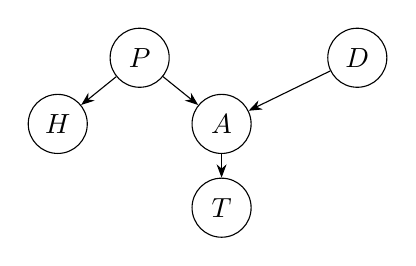
\begin{tikzpicture}[
      node distance=0.3cm and 0.5cm,
      var/.style={circle, draw, minimum size=0.75cm},
      >={Stealth},
    ]
    \node[var] (P) {$P$};
    \node[var, right=2cm of P] (D) {$D$};
    \node[var, below left=of P] (H) {$H$};
    \node[var, below right=of P] (A) {$A$};
    \node[var, below=of A] (T) {$T$};
    \draw[->] (P) -- (H);
    \draw[->] (P) -- (A);
    \draw[->] (D) -- (A);
    \draw[->] (A) -- (T);
  \end{tikzpicture}
  \caption{Causal relations for Problem~\ref{prob:student-network}}
  \label{fig:student-network}
\end{figure}

\begin{solution}
\solpart{Idea}
This problem uses the method of Problem~\ref{prob:medical-test} on a larger graph. The graph in
Figure~\ref{fig:student-network} gives the joint distribution as a product
of one factor for each node. Each factor is the distribution of the node
given its parents:
\[
  p(P, D, A, H, T)
  = p(P) \, p(D) \, p(A \mid P, D) \, p(H \mid P) \, p(T \mid A).
\]
The tables give all five factors. Thus the joint distribution is known,
and you can get any probability from it. To find the probability of $P$
given an observation, move through the graph in two directions:
\begin{enumerate}
  \item Along the edges, from $P$ to the observed variable. Sum over each
    unobserved variable on the path with the chain rule, for example
    $p(T \mid P) = \sum_A p(T \mid A) \, p(A \mid P)$.
  \item Against the edges, from the observed variable back to $P$. Use
    Bayes' theorem, for example
    $p(P \mid T) \propto p(P) \, p(T \mid P)$.
\end{enumerate}

\solpart{Solution}
\solstep{Step 1. Find the probability of a bad answer given the party.}
The depression $D$ is not observed, so sum over $D$. The variables $P$ and
$D$ are source nodes of the graph, so they are independent, and
$p(D \mid P) = p(D)$:
\[
  p(A = 1 \mid P) = \sum_{D} p(A = 1 \mid P, D) \, p(D).
\]
Substitute the values from the tables:
\begin{align*}
  p(A = 1 \mid P = 1) &= 0.999 \cdot 0.4 + 0.9 \cdot 0.6 = 0.9396, \\
  p(A = 1 \mid P = 0) &= 0.9 \cdot 0.4 + 0.01 \cdot 0.6 = 0.366.
\end{align*}

\solstep{Step 2. Find the probability of an unhappy teacher given the party.}
The variable $T$ depends on $P$ only through $A$, so sum over $A$:
\[
  p(T = 1 \mid P)
  = p(T = 1 \mid A = 1) \, p(A = 1 \mid P)
  + p(T = 1 \mid A = 0) \, p(A = 0 \mid P).
\]
Substitute the values from Step~1:
\begin{align*}
  p(T = 1 \mid P = 1) &= 0.95 \cdot 0.9396 + 0.5 \cdot 0.0604 = 0.92282, \\
  p(T = 1 \mid P = 0) &= 0.95 \cdot 0.366 + 0.5 \cdot 0.634 = 0.6647.
\end{align*}

\solstep{Step 3. Find $p(P = 1 \mid H = 1)$.}
Use Bayes' theorem with the table for $p(H \mid P)$:
\[
  p(P = 1 \mid H = 1)
  = \frac{p(P = 1) \, p(H = 1 \mid P = 1)}
         {\sum_{P} p(P) \, p(H = 1 \mid P)}
  = \frac{0.2 \cdot 0.9}{0.2 \cdot 0.9 + 0.8 \cdot 0.2}
  = \frac{0.18}{0.34} \approx 0.529.
\]

\solstep{Step 4. Find $p(P = 1 \mid T = 1)$.}
Use Bayes' theorem with the values from Step~2:
\[
  p(P = 1 \mid T = 1)
  = \frac{0.2 \cdot 0.92282}{0.2 \cdot 0.92282 + 0.8 \cdot 0.6647}
  = \frac{0.184564}{0.716324} \approx 0.258.
\]

\solstep{Step 5. Show that $H$ and $T$ are independent given $P$.}
Sum the joint distribution over the unobserved variables $D$ and $A$. Move
each factor out of the sums that do not contain its variables:
\[
  p(P, H, T)
  = p(P) \, p(H \mid P)
    \sum_{A} p(T \mid A) \sum_{D} p(D) \, p(A \mid P, D)
  = p(P) \, p(H \mid P) \, p(T \mid P).
\]
The last equality uses Steps 1 and 2. Thus
$p(H, T \mid P) = p(H \mid P) \, p(T \mid P)$.

\solstep{Step 6. Find $p(P = 1 \mid T = 1, H = 1)$.}
Use Bayes' theorem with the product from Step~5:
\[
  p(P = 1 \mid T = 1, H = 1)
  = \frac{0.2 \cdot 0.9 \cdot 0.92282}
         {0.2 \cdot 0.9 \cdot 0.92282 + 0.8 \cdot 0.2 \cdot 0.6647}
  = \frac{0.16611}{0.27246} \approx 0.610.
\]

\solpart{Conclusion}
The prior probability of the party is 0.2. A headache increases it to
0.529. An unhappy teacher increases it only to 0.258, because a bad answer
has other causes, and the teacher is often unhappy without a bad answer.
The two observations together give the highest probability, 0.610.
\end{solution}

  \item Let $x_1 \sim \Poiss(\lambda_1)$ and $x_2 \sim \Poiss(\lambda_2)$ be two
independent Poisson random variables, that is,
$p(x_i = k) = \exp(-\lambda_i) \frac{\lambda_i^k}{k!}$,
$k = 0, 1, 2, \ldots$ Prove that
$x_1 + x_2 \sim \Poiss(\lambda_1 + \lambda_2)$.

\begin{solution}
\solpart{Idea}
To find the distribution of a function $y = f(x_1, \ldots, x_n)$ of discrete
random variables, find $p(y = k)$ for each value $k$:
\begin{enumerate}
  \item Write the event $\{f(x_1, \ldots, x_n) = k\}$ as a union of
    disjoint events $\{x_1 = j_1, \ldots, x_n = j_n\}$, one for each tuple
    with $f(j_1, \ldots, j_n) = k$.
  \item The probability of a union of disjoint events is the sum of their
    probabilities:
    \[
      p(y = k) = \sum_{f(j_1, \ldots, j_n) = k}
        p(x_1 = j_1, \ldots, x_n = j_n).
    \]
  \item If the variables are independent, write each joint probability as
    a product.
  \item Simplify the sum and compare it with known distributions.
\end{enumerate}

\solpart{Solution}
\solstep{Step 1. Write the event as a union of disjoint events.}
The variables take only the values $0, 1, 2, \ldots$ Thus $x_1 + x_2 = k$ if
and only if $x_1 = j$ and $x_2 = k - j$ for one $j \in \{0, \ldots, k\}$:
\[
  \{x_1 + x_2 = k\} = \bigcup_{j=0}^{k} \{x_1 = j, \ x_2 = k - j\}.
\]
The events are disjoint, because each event has a different value of $x_1$.

\solstep{Step 2. Sum the probabilities of the disjoint events.}
\[
  p(x_1 + x_2 = k) = \sum_{j=0}^{k} p(x_1 = j, \ x_2 = k - j).
\]

\solstep{Step 3. Use the independence of $x_1$ and $x_2$.}
\[
  p(x_1 + x_2 = k) = \sum_{j=0}^{k} p(x_1 = j) \, p(x_2 = k - j).
\]

\solstep{Step 4. Substitute the Poisson probabilities.}
\[
  p(x_1 + x_2 = k)
  = \sum_{j=0}^{k} e^{-\lambda_1} \frac{\lambda_1^j}{j!} \cdot
    e^{-\lambda_2} \frac{\lambda_2^{k-j}}{(k-j)!}.
\]

\solstep{Step 5. Move the factors that do not depend on $j$ out of the sum.}
\[
  p(x_1 + x_2 = k)
  = e^{-\lambda_1} e^{-\lambda_2}
    \sum_{j=0}^{k} \frac{\lambda_1^j \lambda_2^{k-j}}{j! \, (k-j)!}
  = e^{-(\lambda_1 + \lambda_2)}
    \sum_{j=0}^{k} \frac{\lambda_1^j \lambda_2^{k-j}}{j! \, (k-j)!}.
\]

\solstep{Step 6. Multiply and divide by $k!$.}
\[
  p(x_1 + x_2 = k)
  = \frac{e^{-(\lambda_1 + \lambda_2)}}{k!}
    \sum_{j=0}^{k} \frac{k!}{j! \, (k-j)!} \lambda_1^j \lambda_2^{k-j}
  = \frac{e^{-(\lambda_1 + \lambda_2)}}{k!}
    \sum_{j=0}^{k} \binom{k}{j} \lambda_1^j \lambda_2^{k-j}.
\]

\solstep{Step 7. Use the binomial theorem.}
The binomial theorem gives
$\sum_{j=0}^{k} \binom{k}{j} \lambda_1^j \lambda_2^{k-j}
= (\lambda_1 + \lambda_2)^k$. Thus
\[
  p(x_1 + x_2 = k)
  = e^{-(\lambda_1 + \lambda_2)} \frac{(\lambda_1 + \lambda_2)^k}{k!}.
\]
This is the probability mass function of
$\Poiss(\lambda_1 + \lambda_2)$.

\solpart{Conclusion}
The sum of two independent Poisson random variables is a Poisson random
variable, and the parameters add. By induction, the same is true for any
finite number of independent Poisson random variables.
\end{solution}

  \item \label{prob:poisson-mle}
Let $x_1, x_2, \ldots, x_N$ be an independent sample from $\Poiss(\lambda)$.
Find the maximum likelihood estimate of $\lambda$.

  \item \label{prob:poisson-gamma}
Let $x_1, x_2, \ldots, x_N$ be an independent sample from $\Poiss(\lambda)$.
The prior distribution is the gamma distribution
\[
  p(\lambda) = \Gam(\lambda \mid a, b)
  = \frac{b^a}{\Gamma(a)} \lambda^{a - 1} \exp(-b \lambda),
  \quad a, b > 0.
\]
Find the Bayesian estimate of $\lambda$ as the mean of the posterior
distribution $p(\lambda \mid x_1, \ldots, x_N)$.

\begin{solution}
\solpart{Idea}
The numerator and the denominator of Bayes' theorem contain the same
function:
\[
  p(\lambda \mid X)
  = \frac{p(X \mid \lambda) \, p(\lambda)}
         {\int p(X \mid \lambda) \, p(\lambda) \, d\lambda},
  \qquad X = (x_1, \ldots, x_N).
\]
Do not calculate the integral directly:
\begin{align*}
  p(X \mid \lambda) \, p(\lambda) &= C \cdot g(\lambda)
    && \text{($C$ does not depend on $\lambda$)} \\
  g(\lambda) &= Z \, q(\lambda)
    && \text{($q$ is a known density)} \\
  \int C Z \, q(\lambda) \, d\lambda &= C Z
    && \text{(a density integrates to 1)} \\
  p(\lambda \mid X) &= \frac{C Z \, q(\lambda)}{C Z} = q(\lambda).
\end{align*}
The same method gives the posterior mean.

\solpart{Solution}
Let $S = \sum_{i=1}^{N} x_i$, $a' = a + S$, and $b' = b + N$.

\solstep{Step 1. Write the goal.}
\[
  \hat{\lambda}_{\mathrm{B}} = \mathbb{E}[\lambda \mid X]
  = \int \lambda \, p(\lambda \mid X) \, d\lambda.
\]

\solstep{Step 2. Find $p(\lambda \mid X)$ for Step 1.}
\[
  p(\lambda \mid X)
  = \frac{p(X \mid \lambda) \, p(\lambda)}
         {\int p(X \mid \lambda) \, p(\lambda) \, d\lambda}.
\]

\solstep{Step 2a. Separate the constant in the numerator of Step 2.}
\begin{align*}
  p(X \mid \lambda) \, p(\lambda)
  &= \prod_{i=1}^{N} e^{-\lambda} \frac{\lambda^{x_i}}{x_i!}
     \cdot \frac{b^a}{\Gamma(a)} \lambda^{a-1} e^{-b\lambda}
   = \frac{e^{-N\lambda} \lambda^{S}}{\prod_{i} x_i!}
     \cdot \frac{b^a}{\Gamma(a)} \lambda^{a-1} e^{-b\lambda} \\
  &= \underbrace{\frac{b^a}{\Gamma(a) \prod_{i} x_i!}}_{C}
     \cdot
     \underbrace{\lambda^{a' - 1} e^{-b'\lambda}}_{g(\lambda)}.
\end{align*}

\solstep{Step 2b. Find the known density for $g$ from Step 2a.}
\[
  \Gam(\lambda \mid a', b')
  = \frac{b'^{a'}}{\Gamma(a')} \lambda^{a' - 1} e^{-b'\lambda}
  \;\Longrightarrow\;
  g(\lambda) = \frac{\Gamma(a')}{b'^{a'}} \, \Gam(\lambda \mid a', b').
\]

\solstep{Step 2c. Substitute Steps 2a and 2b into Step 2.}
\[
  p(\lambda \mid X)
  = \frac{C \frac{\Gamma(a')}{b'^{a'}} \, \Gam(\lambda \mid a', b')}
         {C \frac{\Gamma(a')}{b'^{a'}}
          \int \Gam(\lambda \mid a', b') \, d\lambda}
  = \frac{C \frac{\Gamma(a')}{b'^{a'}} \, \Gam(\lambda \mid a', b')}
         {C \frac{\Gamma(a')}{b'^{a'}}}
  = \Gam(\lambda \mid a + S, \, b + N).
\]

\solstep{Step 3. Substitute Step 2c into Step 1.}
\[
  \mathbb{E}[\lambda \mid X]
  = \int \lambda \, \Gam(\lambda \mid a', b') \, d\lambda
  = \frac{b'^{a'}}{\Gamma(a')} \int \lambda^{a'} e^{-b'\lambda} \, d\lambda.
\]

\solstep{Step 3a. Find the integral for Step 3 with the same method.}
\[
  \lambda^{a'} e^{-b'\lambda}
  = \frac{\Gamma(a' + 1)}{b'^{a' + 1}} \, \Gam(\lambda \mid a' + 1, b')
  \;\Longrightarrow\;
  \int \lambda^{a'} e^{-b'\lambda} \, d\lambda
  = \frac{\Gamma(a' + 1)}{b'^{a' + 1}}.
\]

\solstep{Step 3b. Substitute Step 3a into Step 3.}
\begin{align*}
  \mathbb{E}[\lambda \mid X]
  &= \frac{b'^{a'}}{\Gamma(a')} \cdot \frac{\Gamma(a' + 1)}{b'^{a' + 1}}
   = \frac{a' \, \Gamma(a')}{\Gamma(a') \, b'}
     && \text{($\Gamma(a' + 1) = a' \, \Gamma(a')$)} \\
  &= \frac{a'}{b'} = \frac{a + S}{b + N}.
\end{align*}
\[
  \hat{\lambda}_{\mathrm{B}} = \frac{a + S}{b + N}.
\]

\solpart{Conclusion}
\begin{itemize}
  \item \emph{Conjugate prior:} gamma prior $\times$ Poisson likelihood
    $\to$ gamma posterior. The update only changes the parameters:
    $a \to a + S$ (events), $b \to b + N$ (observations).
  \item The estimate is a weighted mean of the prior mean and the
    estimate $\bar{x}$ from Problem~\ref{prob:poisson-mle}:
    \[
      \frac{a + S}{b + N}
      = \frac{a}{b + N} + \frac{S}{b + N}
      = \frac{b}{b + N} \cdot \frac{a}{b}
      + \frac{N}{b + N} \cdot \bar{x}
      \;\xrightarrow{N \to \infty}\; \bar{x}.
    \]
  \item If $a, b \to 0$, then $p(\lambda) \propto \lambda^{a - 1}
    e^{-b\lambda} \to 1/\lambda$, the non-informative prior from the notes
    below, and $\hat{\lambda}_{\mathrm{B}} \to S/N = \bar{x}$.
\end{itemize}
\end{solution}

\paragraph{Notes on comparing the estimates from
  Problems~\ref{prob:poisson-mle} and~\ref{prob:poisson-gamma}.}
\begin{enumerate}[label=\arabic*.]
  \item For more about non-informative priors, see Section~5.4 ``Priors''
    in Kevin P.\ Murphy, \emph{Machine Learning: A Probabilistic
    Perspective}.
  \item The prior $p(\lambda) \propto \frac{1}{\lambda}$ is a uniform prior
    on $\log \lambda$. To see this, use the change-of-variables rule for
    the density of a function of a random variable. See, for example,
    \href{https://en.wikipedia.org/wiki/Probability_density_function#Function_of_random_variables_and_change_of_variables_in_the_probability_density_function}{this
    article}.
\end{enumerate}

\end{enumerate}

\end{document}
